\documentclass{beamer}

\mode<presentation> {
    \usepackage[utf8]{inputenc}
    \usepackage[T1]{fontenc}
    \usepackage[english]{babel}
    \usepackage{csquotes}
    \usepackage{ragged2e} 

    \bibliographystyle{plain}

    \usetheme{Madrid}
    \usecolortheme{ipbutfpr}

    % Can change the colors at beamercolorthemeipbutfpr.sty
    %\setbeamersize{text margin left=0.6cm,text margin right=0.6cm}
    \setbeamertemplate{caption}[numbered]
    \setbeamertemplate{bibliography item}{\insertbiblabel}
    \setbeamertemplate{frametitle continuation}{\gdef\beamer@frametitle{}\justifying}

    \setbeamertemplate{footline}{
        \leavevmode%
        \hbox{%
            \begin{beamercolorbox}[wd=.5\paperwidth,ht=2.25ex,dp=1ex,center]{author in head/foot}%
                \usebeamerfont{author in head/foot}\insertshortauthor
            \end{beamercolorbox}%
            \begin{beamercolorbox}[wd=.5\paperwidth,ht=2.25ex,dp=1ex,center]{title in head/foot}%
                \hspace*{7em}\usebeamerfont{title in head/foot}\insertshorttitle\hspace*{7em}
                \insertframenumber{} / \inserttotalframenumber\hspace*{1ex}
            \end{beamercolorbox}
        }%
        \vskip0pt%
    }

    \setbeamertemplate{navigation symbols}{}
}

\usepackage{amsmath}
\usepackage{amssymb}
\usepackage[language=english, style=numeric, sorting=none]{biblatex}
\usepackage[makeroom]{cancel}

\addbibresource{main.bib}
\makeatletter
\makeatother

\title{\textbf{Graver Basis}}
%\subtitle{A short story}

\author{\textbf{Francisco Javier Blázquez Martínez}}

\institute[EPFL]{\normalsize
    % TODO: How should this be?
    % Prof. Friedrich Eisenbrand \\
    % Jana Cslovjecsek \\

    \begin{figure}[htb]
        % TODO: Maybe shift it a little bit to the right
        \centering
        
\includegraphics[width=0.4\textwidth]{images/logos/epfl_logo.png}
    \end{figure}
}

% TODO: Chair of discrete optimization is maybe too much
\date{\small Department of discrete optimization \\ November 2020}

\begin{document}
    \justifying
    
    \frame{\titlepage}
    
    % TODO: Index or not necessary?
    %\begin{frame}
    %\frametitle{Table of Contents}
    %\tableofcontents
    %\end{frame}

    %\begin{frame}
    %\frametitle{Abstract}
    
    %In this presentation we introduce the concept of \textit{Graver basis}, their main properties, bounds, and a general IP algorithm based on these. We also introduce the N-Fold IP as an example of success applying Graver basis related techniques.
        
    %\end{frame}
    
    \section{Integer Linear Programming}
    \begin{frame}
        \frametitle{Integer Linear Programming}
        \begin{equation*}
            (IP) \equiv max\{c^tx : Ax = b, l \leq x \leq u, x \in \mathbb{Z}^n \}
        \end{equation*}
        \begin{center}
        $A \in \mathbb{Z}^{mxn}$, $b \in \mathbb{Z}^m$, $c \in \mathbb{Z}^n$, $l$  and $u$ lower and upper bounds for x
        \end{center}
        
        
        %\pause
        \vspace{1cm}
        \begin{itemize}
            \item NP-Hard
            \pause
            \item Cutting plane methods
            \item Lattice-basis reduction
            \item Dynamic programming
            \item \alert{Graver basis} techniques
        \end{itemize}
        
        %IP is NP-Hard. There are algorithms with polynomial complexity for certain IPs and there are algorithms for the general IPs based on cutting plane methods, dinamic programming, lattice-basis reduction... 
        
        %\vspace{0.8cm}
        %Thanks to the study of \textbf{Graver basis} new algorithms have appeared improving classic techniques in certain cases. 
        
        
        
    \end{frame}
    
    \begin{frame}
        \frametitle{Integer Linear Programming}
        
        \begin{columns}[T] % align columns
        \begin{column}{.48\textwidth}
        %\color{red}\rule{\linewidth}{4pt}
        \begin{equation*}
            (P1) \equiv 	\left( \begin{array}{l}
	                        \qquad \max \hspace{2pt}  6x + y  \vspace{4pt} \\ 
	                        s.t: 4x + y \leq 19 \\
	                        \qquad x + 2y \leq 31 \\
	                        \qquad x,y\geq 0 \\
	                        \qquad x,y \in \mathbb{Z}
	                        \end{array} \right)
        \end{equation*}
        %\begin{itemize}
            %\item<1-> Text visible on slide 1
            %\item<2-> Text visible on slide 2
            %\item<3> Text visible on slide 3
            %\item<4-> Text visible on slide 4
            %\item Feasible region
            %\item Extreme points
            %\item Directions
            %\item Extreme directions
        %\end{itemize}
        \end{column}%
        \hfill%
        \begin{column}{.48\textwidth}
            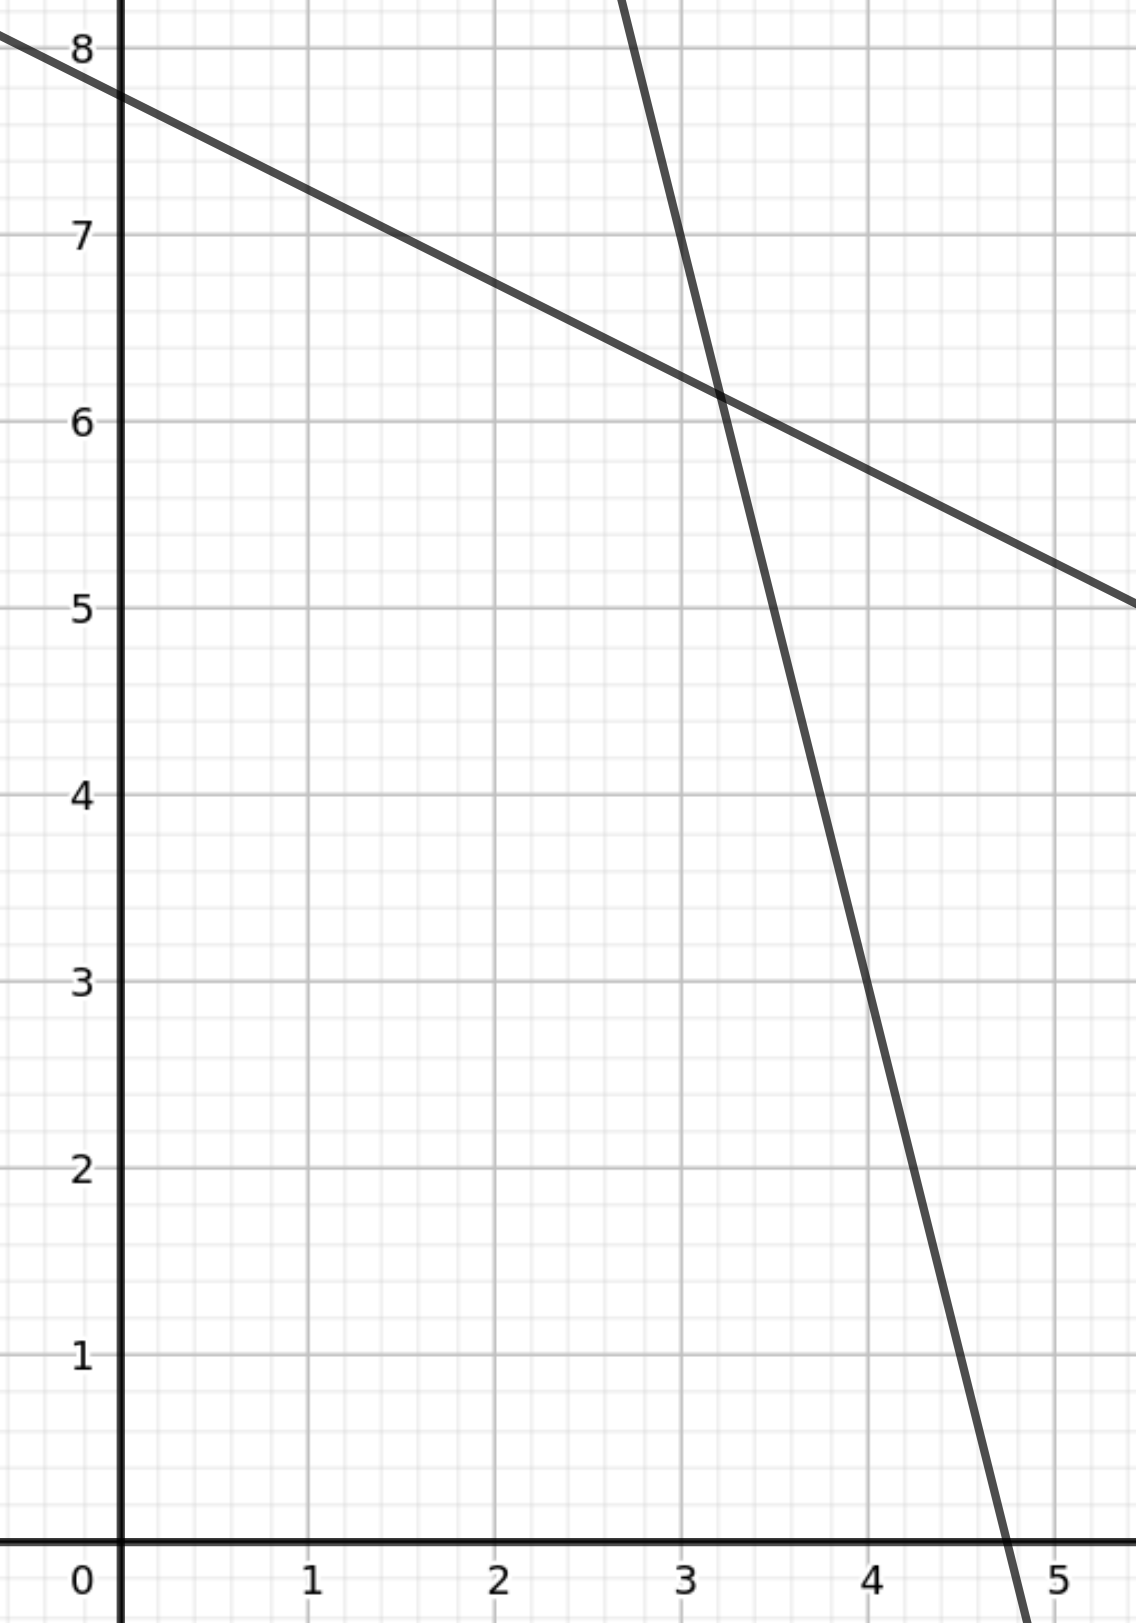
\includegraphics[width=0.85\textwidth]{images/IP(13).png}
        \end{column}%
        \end{columns}
        
        %\addtocounter{framenumber}{-1}

    \end{frame}
    
        \begin{frame}
        \frametitle{Integer Linear Programming}
        
        \begin{columns}[T] % align columns
        \begin{column}{.48\textwidth}
        %\color{red}\rule{\linewidth}{4pt}
        \begin{equation*}
            (P1) \equiv 	\left( \begin{array}{l}
	                        \qquad \max \hspace{2pt}  6x + y  \vspace{4pt} \\ 
	                        s.t: 4x + y \leq 19 \\
	                        \qquad x + 2y \leq 31 \\
	                        \qquad x,y\geq 0 \\
	                        \qquad \xcancel{x,y \in \mathbb{Z}}
	                        \end{array} \right)
        \end{equation*}
        \begin{itemize}
            %\item<1-> Text visible on slide 1
            %\item<2-> Text visible on slide 2
            %\item<3> Text visible on slide 3
            %\item<4-> Text visible on slide 4
            \item Feasible region
            \item Extreme points
            \item Optimum in extreme points
        \end{itemize}
        \end{column}%
        \hfill%
        \begin{column}{.48\textwidth}
            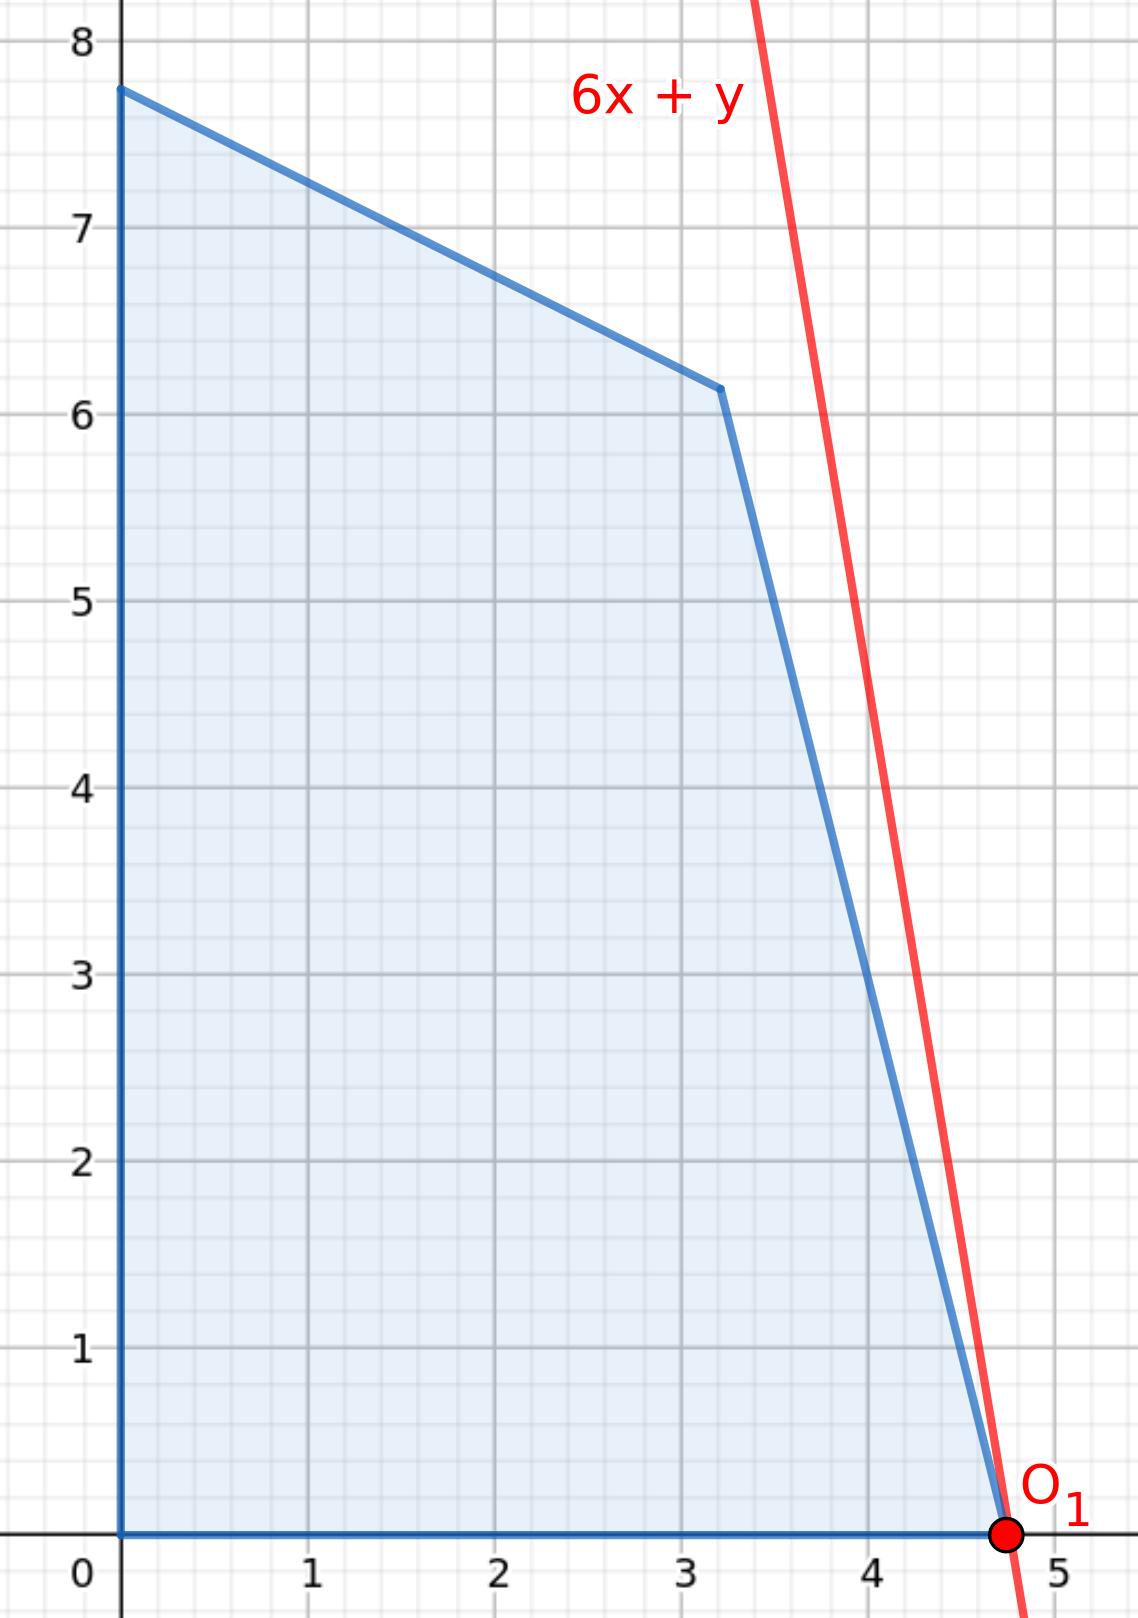
\includegraphics[width=0.85\textwidth]{images/IP(3).png}
        \end{column}%
        \end{columns}
        
        \addtocounter{framenumber}{-1}

    \end{frame}
    
        \begin{frame}
        \frametitle{Integer Linear Programming}
        
        \begin{columns}[T] % align columns
        \begin{column}{.48\textwidth}
        %\color{red}\rule{\linewidth}{4pt}
        \begin{equation*}
            (P1) \equiv 	\left( \begin{array}{l}
	                        \qquad \max \hspace{2pt}  6x + y  \vspace{4pt} \\ 
	                        s.t: 4x + y \leq 19 \\
	                        \qquad x + 2y \leq 31 \\
	                        \qquad x,y\geq 0 \\
	                        \qquad x,y \in \mathbb{Z}
	                        \end{array} \right)
        \end{equation*}
        \begin{itemize}
            \item Feasible points
            \item Optimum can be far from the linear relaxation solution.
        \end{itemize}
        \end{column}%
        \hfill%
        \begin{column}{.48\textwidth}
            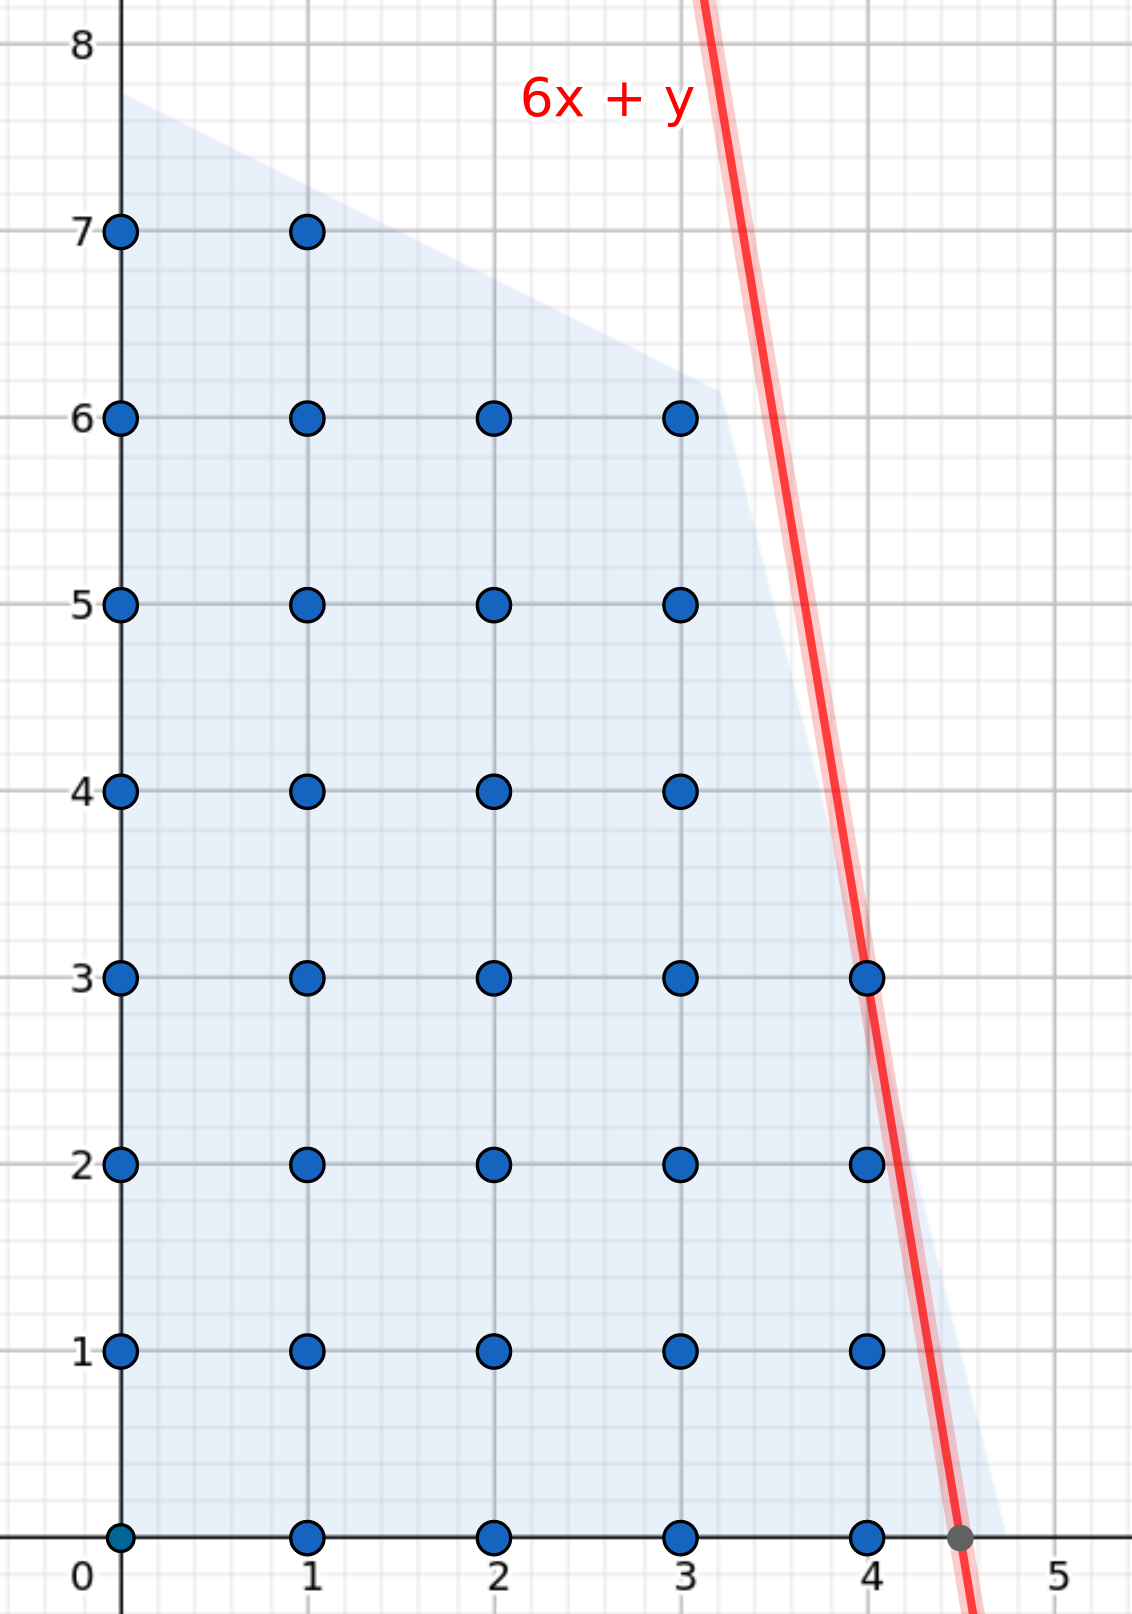
\includegraphics[width=0.85\textwidth]{images/IP(2).png}
        \end{column}%
        \end{columns}
        
        \addtocounter{framenumber}{-1}

    \end{frame}
    
        \begin{frame}
        \frametitle{Integer Linear Programming}
        
        \begin{columns}[T] % align columns
        \begin{column}{.48\textwidth}
        %\color{red}\rule{\linewidth}{4pt}
        \begin{equation*}
            (P1) \equiv 	\left( \begin{array}{l}
	                        \qquad \max \hspace{2pt}  6x + y  \vspace{4pt} \\ 
	                        s.t: 4x + y \leq 19 \\
	                        \qquad x + 2y \leq 31 \\
	                        \qquad x,y\geq 0 \\
	                        \qquad \xcancel{x,y \in \mathbb{Z}}
	                        \end{array} \right)
        \end{equation*}
        \begin{itemize}
            %\item<1-> Text visible on slide 1
            %\item<2-> Text visible on slide 2
            %\item<3> Text visible on slide 3
            %\item<4-> Text visible on slide 4
            \item Extreme directions: \\
            Allow Simplex fast optimality test and finding a direction of improvement in LP. 
            
            \vspace{0.5cm}
            Can we do the same for IP?
        \end{itemize}
        \end{column}%
        \hfill%
        \begin{column}{.48\textwidth}
            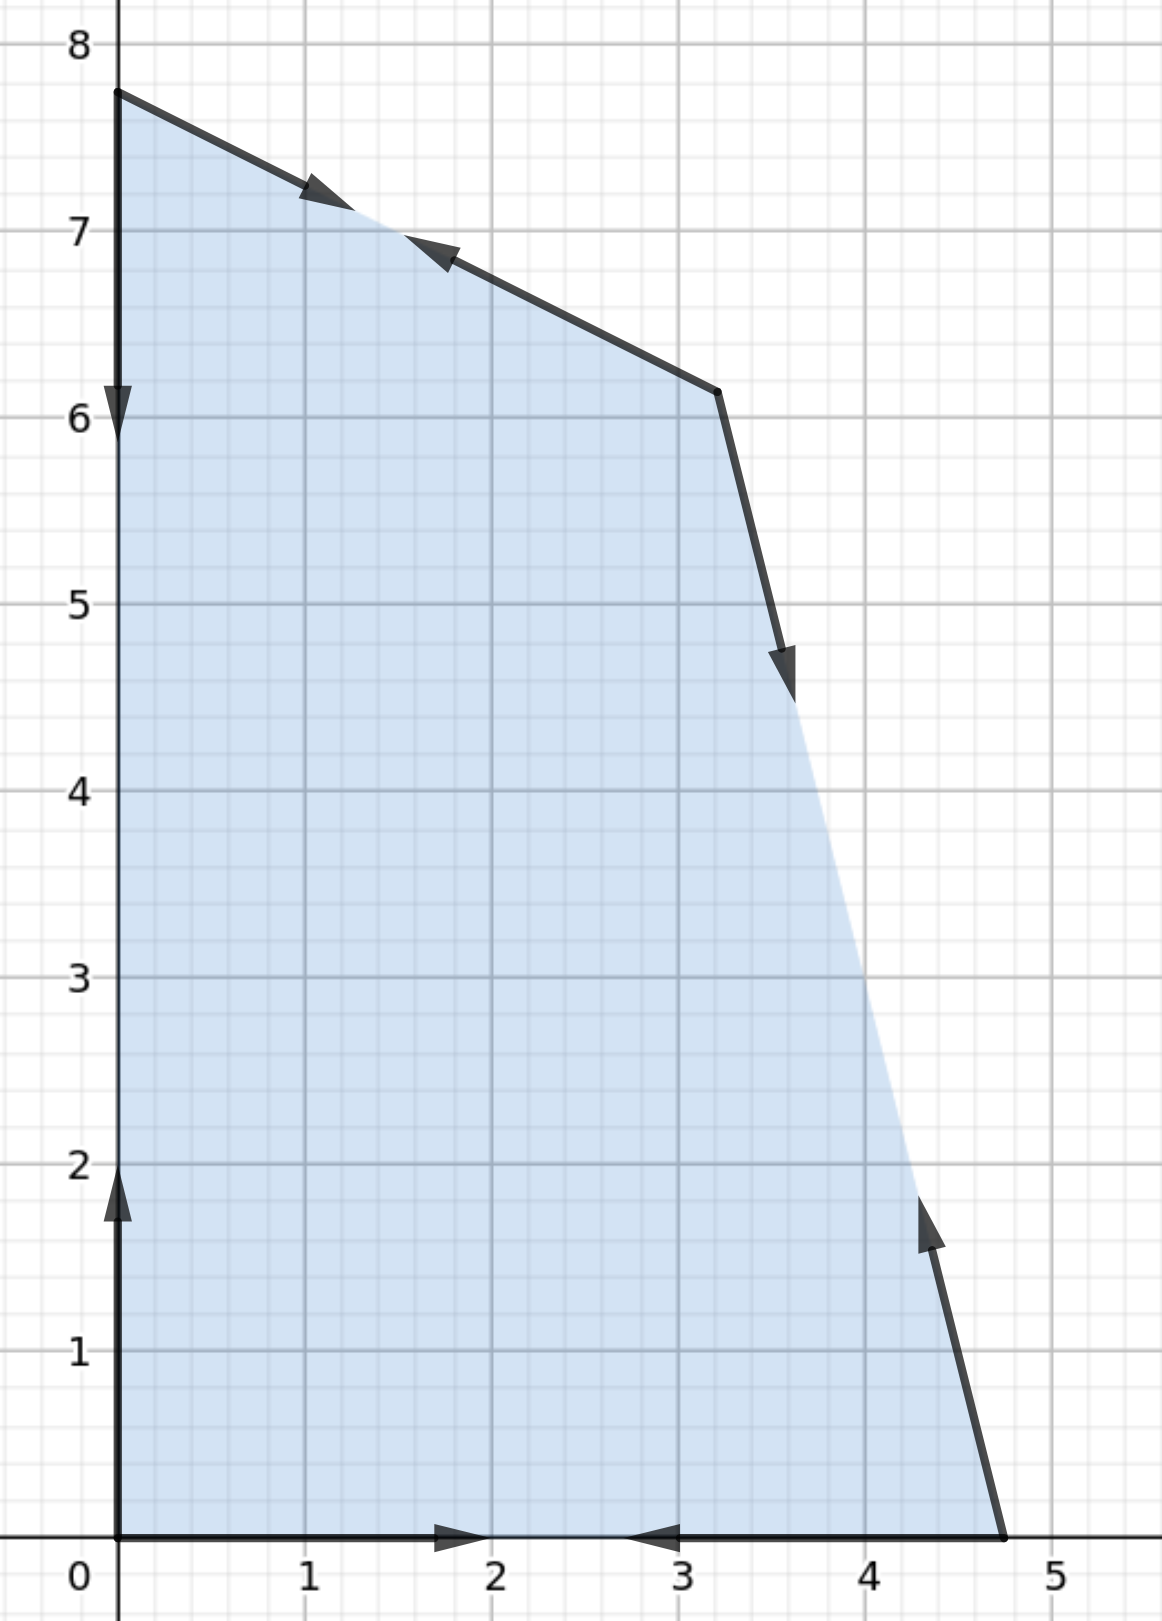
\includegraphics[width=0.85\textwidth]{images/IP(4).png}
        \end{column}%
        \end{columns}
        
        \addtocounter{framenumber}{-1}

    \end{frame}

    \section{Graver Basis, definition and properties}
    \begin{frame}
        \frametitle{Graver Basis}
        \begin{itemize}
            \item \textbf{Definition:} Two vectors $u,v \in \mathbb{R}^n$ are said to be \textbf{sign compatible} if $u_i \cdot v_i \geq 0$ for all $i \in \{1,...,n\}$
            \vspace{0.2cm}
            %\pause
            \item \textbf{Definition:} A vector $u \in ker(A)$ is \textbf{indecomposable} if it is not the sum of two sign compatible and non zero elements in $ker(A)$.
            %\pause
        \end{itemize}
        
        \pause
        \vspace{1cm}
        \begin{block}{Graver Basis $\equiv Gr(A)$ }
            The Graver Basis of a given matrix A is defined as the set of integral indecomposable elements in the kernel of A.
        \end{block}
        (Initially defined as \textit{universal integral test set} in [Graver 1975])
    \end{frame}
    
    \begin{frame}
        \frametitle{Graver Basis properties}
        \begin{itemize}
            \justifying
            \item \textbf{Spanning:} Every integral element in ker(A) can be expressed as positive integral linear combination of elements in $Gr(A)$.
        \end{itemize}
        
        \vspace{0.5cm}
        \begin{itemize}
            \justifying
            \item \textbf{Optimality:} Given z in the feasible region of an IP, z is not optimum if and only if there exists $g \in Gr(A)$ s.t. $c^tg > 0$ and $l \leq z + g \leq u$
            %\pause
        \end{itemize}
        
        
        \pause
        \vspace{0.5cm}
        \begin{itemize}
            \justifying
            \item \textbf{Bounds:} Given $A \in \mathbb{Z}^{mxn}$ and $\Delta$ an upper bound for the absolute value of each component of $A$, for every $g \in Gr(A)$:
            \begin{itemize}
                \item $||g||_1 \leq m^{m/2}\Delta^m\cdot(n - m)$ \hspace{10pt}[Onn 2010]
                \item $||g||_1 \leq (2m \Delta + 1)^m$ \hspace{35pt}[Eisenbrand,Hunkenschröder,Klein 2018]
            \end{itemize}
            %\pause
        \end{itemize}

        
    \end{frame}
    
    \begin{frame}
        \frametitle{Graver Basis properties}
        
        \begin{columns}[T] % align columns
        \begin{column}{.48\textwidth}
        %\color{red}\rule{\linewidth}{4pt}
        \begin{equation*}
            (P1) \equiv 	\left( \begin{array}{l}
	                        \qquad \max \hspace{2pt}  6x + y  \vspace{4pt} \\ 
	                        s.t: 4x + y \leq 19 \\
	                        \qquad x + 2y \leq 31 \\
	                        \qquad x,y\geq 0 \\
	                        \qquad x,y \in \mathbb{Z}
	                        \end{array} \right)
        \end{equation*}
        \begin{itemize}
            \justifying
            %\item<1-> Text visible on slide 1
            %\item<2-> Text visible on slide 2
            %\item<3> Text visible on slide 3
            %\item<4-> Text visible on slide 4
            \item If not optimal, an element in Graver basis is an improvement direction.
            \item If Graver basis bounded, we can restrict our improvement direction search.
        \end{itemize}
        \end{column}%
        \hfill%
        \begin{column}{.48\textwidth}
            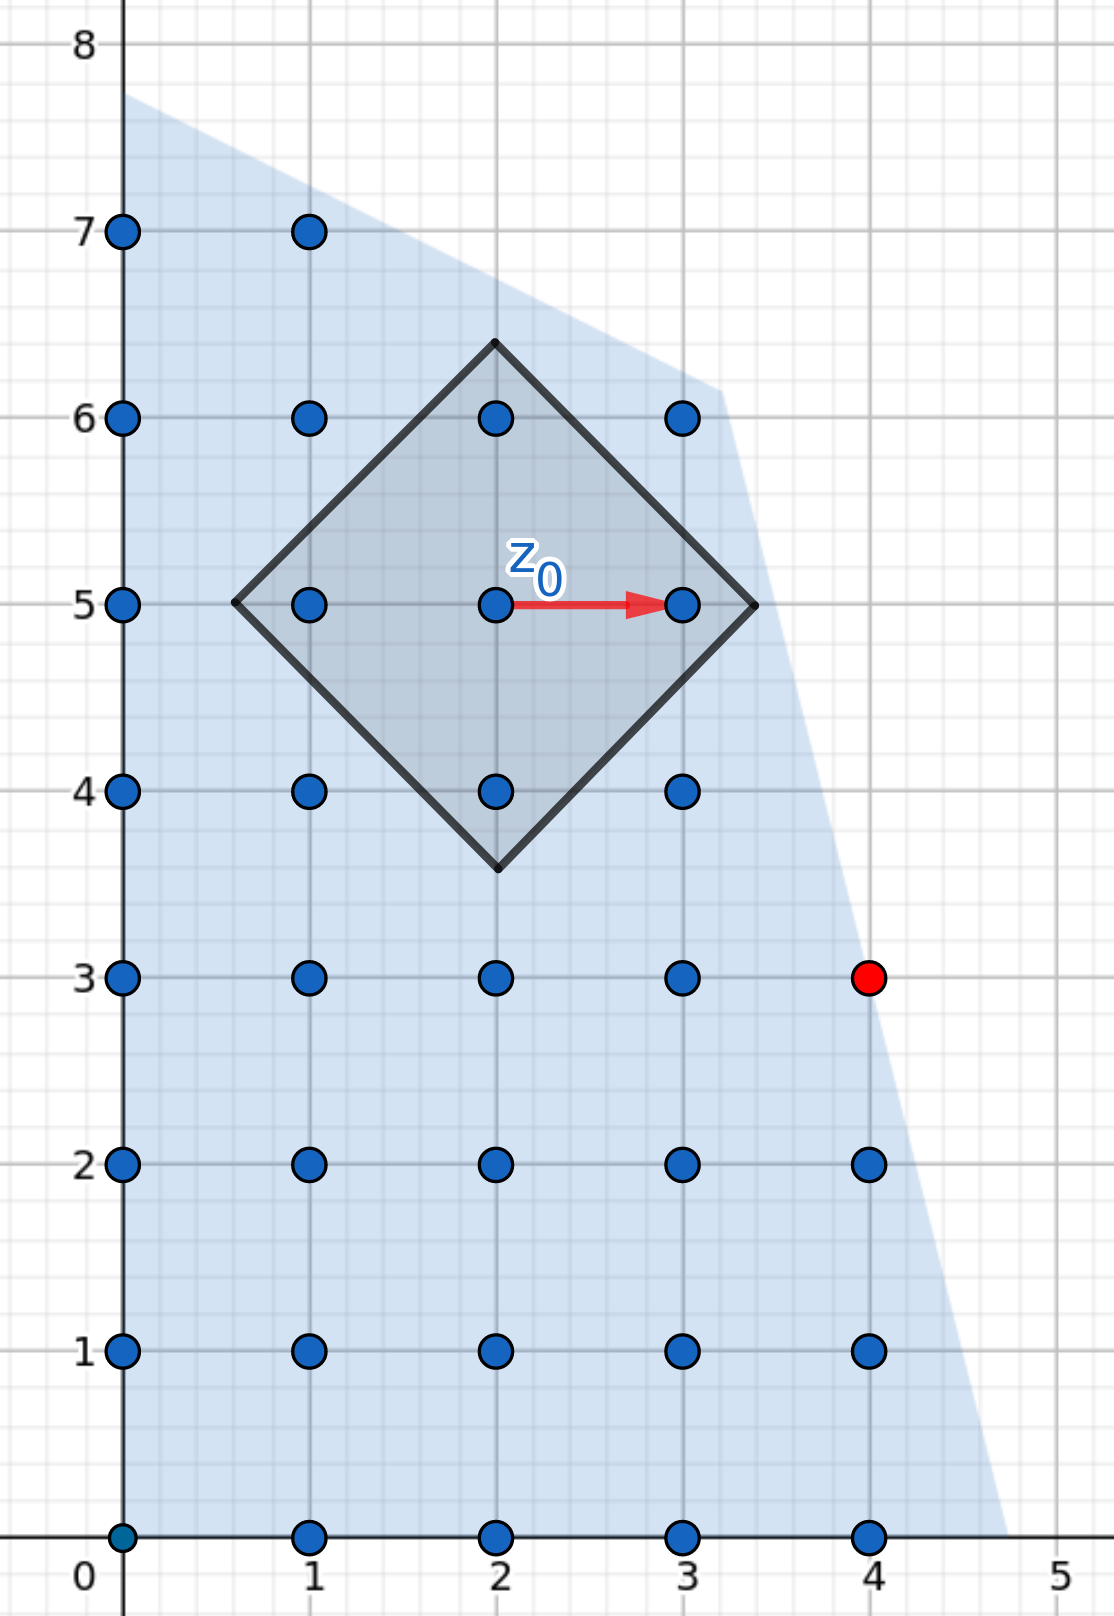
\includegraphics[width=0.85\textwidth]{images/IP(6).png}
        \end{column}%
        \end{columns}
        
        \addtocounter{framenumber}{-1}

    \end{frame}
    
    \begin{frame}
        \frametitle{Augmentation algorithm}
        %The following is a general IP algorithm. At first sight it may not seem an improvement, however, in the sub-problem the feasible region is being restricted to elements bounded by Graver basis norm, which reduces the problem considerably in certain cases. 

        %\vspace{0.5cm}
        %The correctness of this algorithm is given by \textbf{property 2}. 
        %\vspace{0.5cm}
        \begin{block}{\centering General IP algorithm using Graver basis norm bound}
        \begin{enumerate}
            \item From a feasible solution $z_i$
            \item Find $g^*$ optimum for the sub-problem: \vspace{4pt}\\
                  $max\{c^tg : Ag = 0, l-z_i \leq g \leq u-z_i, g \in \mathbb{Z}^n, ||g||_1 \leq ||Gr(A)|| \}$ \vspace{4pt}
            \begin{itemize}
                \item $g^* = 0 \implies z_i$ optimal solution.
                \item $g^* \neq 0 \implies$ $g^*$ improvement direction, loop back to 1 with $z_{i+1} = z_i + \lambda \cdot g^*$ with the biggest $\lambda$ respecting the bounds.
            \end{itemize}
        \end{enumerate}
        \end{block}
        [Hemmecke, Onn, Romanchuk 2013]
    \end{frame}
    
    \section{N-Fold, a success example}
    \begin{frame}
        \frametitle{N-Fold, a success example}
        
        A N-Fold IP has constriction matrix A of the form ($A_i \in \mathbb{Z}^{rxt}, B_i \in \mathbb{Z}^{sxt}$):\\
        \begin{equation*}
        N = 
        \begin{pmatrix}
        A_1 & A_2 & \cdots & A_n \\
        B_1 & 0   & \cdots & 0 \\
        0   & B_2 & \cdots & 0 \\
        \vdots    & \vdots & \ddots & \vdots  \\
        0   & 0   & \cdots & B_n 
        \end{pmatrix}
        \end{equation*}
        
        %\vspace{0.5cm}
        %It's possible (using Steinitz Lemma) to obtain a much tighter bound for the norm of the elements in the Graver basis than the ones mentioned before.
        
        \pause
        \begin{block}{N-Fold Graver basis bound}
            For all $g \in Gr(N)$ $||g||_1 \leq L_B (2r\Delta L_B + 1)^r =: L_A$ where $L_B = (2s \Delta + 1)^s$
        \end{block}
        \pause
        \begin{block}{N-Fold augmentation algorithm complexity}
            The N-Fold IP can be solved in time $n^2t^2\varphi log^2nt \cdot (rs\Delta)^{O(r^2s + rs^2)} + LP$
        \end{block}
        %\addtocounter{framenumber}{-1}
        
        [Eisenbrand, Hunkenschröder, Klein 2018]
    \end{frame}
    
    \begin{frame}
        \frametitle{N-Fold, improving even more}
        
        \begin{figure}[!tbp]
        \centering
        \begin{minipage}[b]{0.45\textwidth}
            \centering
            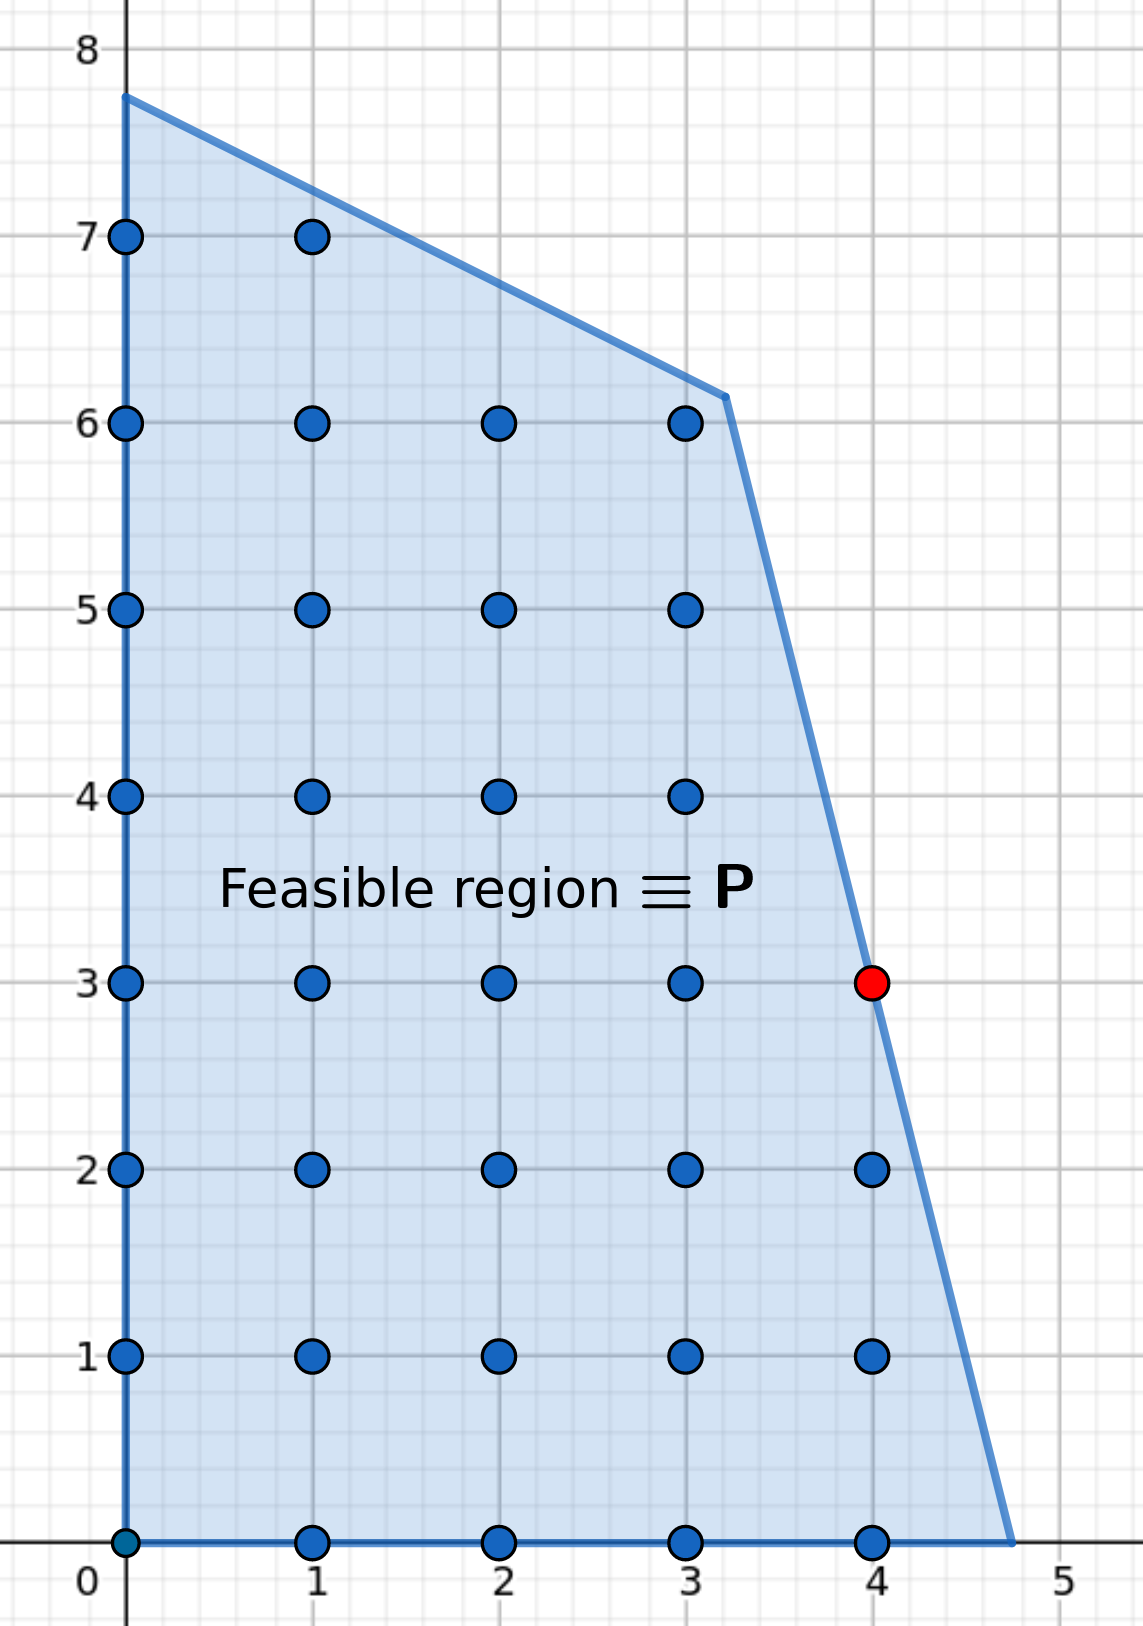
\includegraphics[width=0.9\textwidth]{images/IP(12).png}
            \caption{Linear Relaxation (LR)}
        \end{minipage}
        \hfill
        \begin{minipage}[b]{0.45\textwidth}
            \centering
            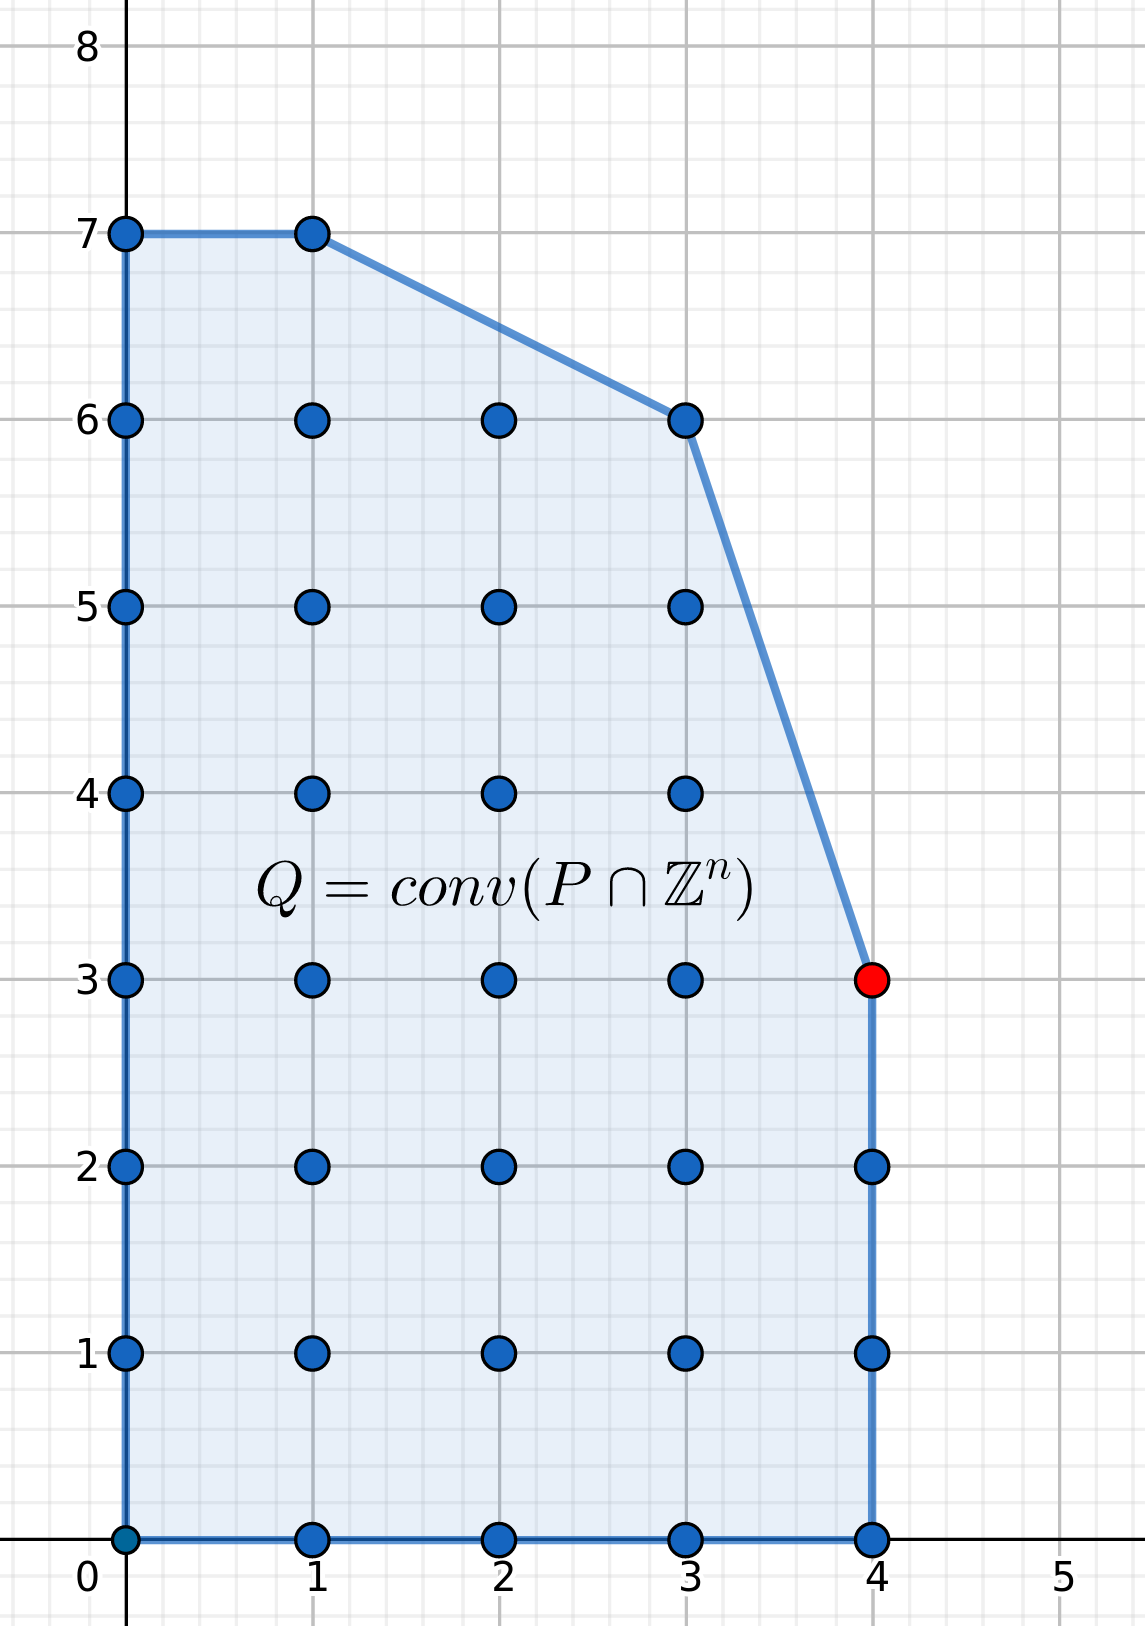
\includegraphics[width=0.9\textwidth]{images/IP(10).png}
            \caption{Restricted LR}
        \end{minipage}
        \end{figure}
    \end{frame}
    \begin{frame}
        \frametitle{N-Fold, improving even more}
        \vspace{0.5cm}
        \begin{block}{N-Fold proximity to restricted LR}
            Let $x^*$ be an optimal vertex solution of a N-Fold IP restricted LR, then there exists an optimal solution for the N-Fold IP verifying:  
            \begin{equation*}
                ||z^* - x^*|| \leq (rs\Delta)^{O(rs)}
            \end{equation*}
        \end{block}
        \pause
        \vspace{0.5cm}
        \begin{block}{N-Fold complexity}
            The N-Fold IP can be solved in time $nt(rs\Delta)^{O(r^2s + s^2)} + LP$
        \end{block}
        [Cslovjecsek, Eisenbrand, Weismantel 2020]
        %\addtocounter{framenumber}{-1}
        
    \end{frame}
    
    
    
    \section{References}
    \begin{frame}[allowframebreaks] % Interesting option!
        \frametitle{References}
        \nocite{*}
        \printbibliography
    \end{frame}

\end{document}
